\chapter{Das Lösungskonzept}
\label{cha:Lösungskonzept}
In diesem Kapitel wird der Lösungsansatz und die Spezifikation des Vorlagenmanagements erörtert. Bei der Spezifikation handelt es sich um Schnittstellen und abstrakte Klassen, die die Struktur des Vorlagenmanagements definieren. Diese Schnittstellen und abstrakten erlauben es Implementierungen für verschiedene \emph{Template-Engines} wie z.B
\begin{itemize}
	\item \emph{Freemakrer},
	\item \emph{Velocity} oder
	\item \emph{Thymeleaf}
\end{itemize}
zur Verfügung zu stellen, wobei die abstrakten Klassen die gemeinsam nutzbare Logik implementieren, die über die verschiedenen \emph{Template-Engines} verwendet werden kann.
\newline
\newline
Mit der Möglichkeit die verschiedensten \emph{Template-Engines} verwenden zu können, wird erreicht dass das Vorlagenmanagement sehr flexibel ist. Bei dem Wechsel zu einer anderen \emph{Template-Engine} müssen nur die \emph{Expressions} einer Vorlagen in die \emph{Template-Engine} spezifischen \emph{Expressions} umgewandelt werden.
\ \newpage

\section{Die Spezifikation des Vorlagenmanagements}
Dieses Kapitel behandelt die erstellten Spezifikationen des Vorlagenmanagements. Auf Basis dieser Spezifikationen wird das Vorlagenmanagement und die Integrationen in die verschiedenen Umgebungen und Technologien implementiert. Die erstellte Spezifikationen sind frei von Abhängigkeiten auf konkrete Implementierungen jeglicher Art. Sie haben nur Abhängigkeiten auf andere Spezifikationen wie die \emph{JEE-7} Spezifikation.

\begin{figure}[h]
\centering
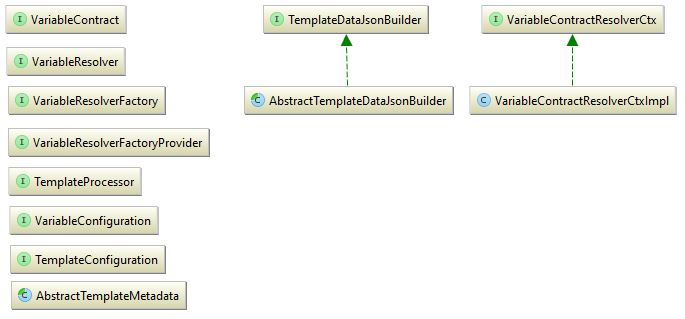
\includegraphics[scale=0.73]{20160710_template-logic-api.jpg} %{CS0031}
\caption{Klassenhierarchie der Vorlagen-\emph{API}}
\label{fig:template-logic-api-hierarchy}
\end{figure}

\subsection{Die Schnittstellen und abstrakten Klassen}
Dieser Abschnitt behandelt die implementierten Schnittstellen und abstrakten Klassen des Vorlagenmanagements. Die abstrakten Klassen implementieren die gemeinsam nutzbaren Funktionalitäten, welche von alle konkreten Implementierungen des Vorlagenmanagements genutzt werden können. Diese Spezifikationen spezifizieren Aspekte des Vorlagenmanagements wie
\begin{enumerate}
	\item das Variablenmanagement innerhalb des Vorlagenmanagement,
	\item die Handhabung von Variablen in einer Vorlage 
	\item die Abbildung der Metadaten einer Voralge und 
	\item das Erstellen des \emph{JSON}-Objekts, welches die Daten für die Vorlage beinhaltet.
\end{enumerate}

\subsubsection{Die Schnittstelle \emph{VariableContract}}
\label{sec:variableContract}
Die Schnittstelle \emph{VariableContract} spezifiziert eine Variable, die in einer Vorlage verwendet werden kann. Objekte dieser Schnittstelle werden beim Anwendungsstart registriert und können grundsätzlich in allen Vorlagen verwendet werden. Eine Variable ist einem Modul zugeordnet, in dem die Variable bezüglich ihres Namen eindeutig sein muss. Das Modul wird über einen \emph{String} definiert. Die Mehrsprachigkeit einer Variable wird über Enumerationen realisiert, wobei jede Variable jeweils einen Schlüssel für den Titel und die Beschreibung bereit stellt. 
\newline
\newline
Da es sich bei einer Variable um statische Daten handelt, also die Variablen sind schon zur Kompilierungszeit bekannt, ist angedacht, dass die Variablen mit dem \emph{Java}-Typ \emph{enum} implementiert werden, dass die Schnittstelle \emph{VariableContract} implementiert. Durch die Abbildung der Variablen mit dem \emph{Java}-Typ \emph{enum} können mehrere Variablen in einer Klasse definiert werden, wobei eine einzelne Enumeration ein Objekt der Schnittstelle \emph{VariableContract} darstellt. Alle Variablen die mit einer \emph{enum} abgebildet werden, sollten demselben Modul zugeordnet sein, obwohl dies nicht zwingend erforderlich ist. Die Zuordnung der Variablen zum selben Modul erleichtert die Wartung und Strukturierung der Variablen. Die Variablen, die mit einer \emph{enum} definiert wurden, werden innerhalb des Vorlagenmanagements trotzdem als einzelne Objekte der Schnittstelle \emph{VariableContract} betrachtet. Die Tatsache dass die Variablen mit einer \emph{enum} abgebildet wurden, ist für das Vorlagenmanagement nur beim Registrieren der Variablen von belang und nicht bei deren weiterer Verwendung.
\newline
\newline
Eine Variable ist über seine \emph{Id} eindeutig referenzierbar, wobei sich die \emph{Id} aus dem Modulnamen und den Variablennamen zusammensetzt (Bsp. module.core.VAR\_1). Die \emph{Id} hält sich dabei an die Namenskonvention eines \emph{Java}-Paketnamen. Da der Variablenname immer auf diese Weise zusammengesetzt werden sollte, wurde die Methode \emph{String getId();} als \emph{default Methode} implementiert, was seit \emph{Java 8} möglich ist. Ein EntwicklerIn muss diese Methode nicht mehr implementieren, obwohl es immer noch möglich ist diese Methode zu überschreiben. Auch die Methode \emph{String toInfoString()} wurde als \emph{default Methode} implementiert, da auch diese Methode nicht von den EntwicklerInnen implementiert werden sollte, da ihre Funktionalität sich nicht ändern sollte.
\newpage

\begin{program}[h]
\caption{VariableContract.java}
\label{prog:variableContract}
\begin{JavaCode}
public interface VariableContract extends Serializable {

    String getName();

    String getModule();

    Enum<?> getInfoKey();

    Enum<?> getLabelKey();

    default String getId() {      
        return getModule() + "." + getName();
    }

    default String toInfoString() {
        final String ls = System.lineSeparator();
        final StringBuilder sb = new StringBuilder();
        sb.append("contract  : ").append(this.getClass().getName())
          .append(ls)
          .append("id        : ").append(getId())
          .append(ls)
          .append("name      : ").append(getName())
          .append(ls)
          .append("label-key : ").append((getLabelKey() != null) 
                                          ? getLabelKey().name() 
                                          : "not available")
          .append(ls)
          .append("info-key  : ").append((getInfoKey() != null) 
                                          ? getInfoKey().name() 
                                          : "not available")
          .append(ls)
          .toString();
    }
}
\end{JavaCode}
\end{program}

\subsubsection{Die Schnittstelle \emph{VariableResolver}}
\label{sec:variableResolver}
Die Schnittstelle \emph{VariableResolver} spezifiziert wie der aktuelle Wert der Variablen aufgelöst wird. Eine Variable wird in einer Vorlage verwendet und beim Erstellen eines Datenbankeintrags, der diese Vorlage verwendet, müssen die aktuellen Werte der beinhalteten Variablen aufgelöst werden. Da der aktuelle Wert der Variable kontextabhängig ist, wird beim Auflösen des Werts der Variable ein Kontext bereitgestellt, über den kontextabhängige Daten vom EntwicklerIn bereitgestellt werden können, die in einer Implementierung der Schnittstelle \emph{VariableResolver} angewendet werden können. Dadurch kann die Variable in mehreren Kontexten verwendet werden und auch kontextabhängig aufgelöst werden.
\begin{program}[h]
\caption{VariableResolver.java}
\label{prog:variableResolver}
\begin{JavaCode}
@FunctionalInterface
public interface VariableResolver {

    String resolve(VariableContract variable,
                   VariableContractResolverContext ctx);
}
\end{JavaCode}
\end{program}
\ \newline
Die Schnittstelle \emph{VariableResolver} wurde als \emph{FunctionalInterface} implementiert. Ein \emph{FunctionalInterface} ist eine Schnittstelle, die nur eine abstrakte Methode definiert, die implementiert werden muss. Eine Implementierung eines \emph{FunctionalInterface} kann über eine \emph{Lambda}-Funktion oder Methodenreferenz bereitgestellt werden, wodurch die Notwendigkeit einer anonymen Implementierung oder der Implementierung einer Klasse für diese Schnittstelle entfällt. Dieser Ansatz macht den Quelltext lesbarer, obwohl angemerkt sei, dass dieser Ansatz sich negativ auf das Laufzeitverhalten auswirkt, was in der Art und Weise der Ausführung einer \emph{Lambda}-Funktion oder Methodenreferenz begründet ist. Die negativen Auswirkungen auf das Laufzeitverhalten können, im Bezug auf das Vorlagenmanagement, vernachlässigt werden.

\subsubsection{Die Schnittstelle \emph{VariableResolverFactory}}
\label{sec:variableResolverFactory}
Die Schnittstelle \emph{VariableResolverFactory} spezifiziert wie Objekte der Schnittstelle \emph{VariableResolver} produziert werden. Objekte dieser Schnittstelle können Objekte der Schnittstelle \emph{VariableResolver} für jede Implementierung der Schnittstelle \emph{VariableContract} produzieren, obwohl es zu empfohlen ist, dass es eine Implementierung der Schnittstelle \emph{VariableResolverFactory} je Modul zur Verfügung gestellt wird.

\begin{program}[h]
\caption{VariableResolverFactory.java}
\label{prog:variableResolverFactory}
\begin{JavaCode}
@FunctionalInterface
public interface VariableResolverFactory extends Serializable {

  VariableResolver getVariableResolver(VariableContract contract,
                                       VariableContractResolverCtx ctx);
}
\end{JavaCode}
\end{program}
\ \newline
Die Schnittstelle \emph{VariableResolver} wurde ebenfalls als \emph{FunctionalInterface} implementiert, damit Implementierungen über eine \emph{Lambda}-Funktion oder eine Methodenreferenz bereitgestellt werden kann.

\subsubsection{Die Schnittstelle \emph{VariableResolverFactoryProvider}}
\label{sec:VariableResolverFactoryProvider}
Die Schnittstelle \emph{VariableContractFactoryProvider} spezifiziert wie Objekte der Schnittstelle \emph{VariableResolverFacotry} produziert werden. Ein Objekt der Schnittstelle \emph{VariableResolverFactoryProvider} kann Objekte der Schnittstelle \emph{VariableResolverFactory} für die Schnittstelle \emph{VariableContract}, einer Ableitung von dieser Schnittstelle oder einer konkreten Implementierung dieser Schnittstelle zur Verfügung stellen. 

\begin{program}[h]
\caption{VariableResolverFactoryProvider.java}
\label{prog:variableResolverFactoryProvider}
\begin{JavaCode}
@FunctionalInterface
public interface VariableResolverFactoryProvider extends Serializable {

    VariableResolverFactory getVariableResolverFactory
            (Class<? extends VariableContract> contractType);
}
\end{JavaCode}
\end{program}
\ \newline
Die Schnittstelle \emph{VariableResolverFactoryProvider} wurde auch als \emph{FunctionalInterface} implementiert um Implementierungen über eine \emph{Lambda}-Funktion oder Methodenreferenz zur Verfügung stellen zu können.

\subsubsection{Die Schnittstelle \emph{VariableContractResolverCtx}}
\label{sec:variableResolverFactoryProvider}
Die Schnittstelle \emph{VariableContractResolverCtx} spezifiziert den Kontext, der bei der beim Auflösen des aktuellen Werts einer Variablen zur Verfügung gestellt wird. Dieser Kontext stellt alle Daten bereit, die beim Auflösen des aktuellen Werts einer Variable benötigt werden. Es wird auch ermöglicht, dass Benutzerdaten im Kontext definiert werden können, die bei beim Auflösen des aktuellen Werts einer Variable verwendet werden können. Es wurde bewusst vermieden, dass beim Auflösen eines aktuellen Werts einer Variable bekannt ist, in welcher Vorlage die Variable verwendet wird. Dadurch bleibt die Handhabung der Variablen einer Vorlage entkoppelt von der Vorlage selbst. Dadurch wäre es möglich die Variablen außerhalb vom Vorlagenmanagements zu verwenden.
\newpage

\begin{program}[h]
\caption{VariableContractResolverCtx.java}
\label{prog:variableContractResolverCtx}
\begin{JavaCode}
public interface VariableContractResolverCtx {

    Locale getLocale();

    ZoneId getZoneId();

    TimeZone getTimeZone();

    <T> T getUserData(Object key,
                      Class<T> clazz);
}
\end{JavaCode}
\end{program}

\subsubsection{Die Schnittstelle \emph{TemplateProcessor}}
\label{sec:templateProcessor}
Die Schnittstelle \emph{TemplateProcessor} spezifiziert wie die Vorlagen behandelt werden. Objekte dieser Schnittstelle können Variablen in einer Vorlage, einer bestimmten \emph{Template-Engine} finden und konvertieren. Ein \emph{TemplateProcessor} muss ebenfalls in der Lage sein ungültige Variablen innerhalb einer Vorlage zu finden, wobei eine ungültige Variable eine Variable ist, die nicht registriert ist und somit auch der aktuelle Wert der Variable nicht aufgelöst werden kann.
\newline
\newline
Eine konkrete Implementierung dieser Schnittstelle ist eine Implementierung für eine bestimmte \emph{Template-Engine}, da die in der Vorlage verwendeten \emph{Expressions} spezifisch für die verwendete \emph{Template-Engine} sind. 
\newline
\newline
Besonders sind beiden folgenden Methoden hervorzuheben.
\begin{JavaCode}[numbers=none]
String replaceExpressions(String template,
                          Function<VariableContract, String> converter);

String replaceCustom(String template,
                     Pattern itemPattern,
                     Function<String, String> converter);
\end{JavaCode}
Diese Methoden verwenden als Formalparameter für den benötigte Konverter ein \emph{FunctionalInterface} namens \emph{Function}, welches von der Sprache \emph{Java 8} bereitgestellt wird. Dadurch ist das Spezifizieren einer eigenen Schnittstelle für die Konvertierung nicht mehr nötig. Der Konverter kann über eine \emph{Lambda}-Funktion oder Methodenreferenz bereitgestellt werden. Dadurch ist die Konvertierung der Variablen einer Vorlage abstrahiert von der Implementierung der Schnittstelle \emph{TemplateProcessor}, wodurch die Variablen durch eine beliebige Repräsentation ersetzt werden können und visa versa.
\newpage

\begin{program}[h]
\caption{TemplateProcessor.java}
\label{prog:templateProcessor}
\begin{JavaCode}
public interface TemplateProcessor {

    String replaceExpressions(String template,
                              Function<VariableContract, String> converter);

    String replaceCustom(String template,
                         Pattern itemPattern,
                         Function<String, String> converter);

    Set<VariableContract> resolveExpressions(String template);

    Set<String> resolveInvalidExpressions(String template);

    String variableToExpression(VariableContract contract);

    VariableContract expressionToVariable(String expression);
}
\end{JavaCode}
\end{program}

\subsubsection{Die Schnittstelle \emph{TemplateDataJsonBuilder}}
\label{sec:templateDataJsonBuilder}
Die Schnittstelle \emph{TemplateDataJsonBuilder} spezifiziert die Signatur eines \emph{Builders}, der das \emph{JSON}-Objekt erstellt, welches die Daten für das Parsen einer Vorlage enthält. Eine Anforderung ist es, die \emph{E-Mail}-Nachrichten persistent zu halten, wobei nach der Erstellung einer \emph{E-Mail}-Nachricht, dessen Inhalt unveränderbar sein soll. Es werden die Metadaten wie die Sprache sowie die aufgelösten Werte der in der Vorlage enthaltenen Variablen mit einem \emph{JSON}-Objekt persistent gehalten. Es könnte auch die Vorlage geparst werden und die gesamte geparste Vorlage persistent gehalten werden, wodurch aber die Menge an persistent gehaltenen Daten stark ansteigen würde. Da nur die Metadaten und die Werte der Variablen persistent gehalten werden, wird die Menge an persistent gehaltenen Daten so klein wie möglich gehalten, da nur die variablen Teile einer Vorlage für eine \emph{E-Mail}-Nachricht persistent gehalten werden. Mit diesem \emph{JSON}-Objekt kann die korrespondierende Vorlage zu jedem Zeitpunkt mit demselben Resultat erneut geparst werden.
\newline
\newline
Es wurde hier das \emph{Builder}-Muster angewendet, da sich die Konfiguration des \emph{Builders} mit einer \emph{Fluent-API}, wie bei einem \emph{Builder} üblich, sehr gut abbilden lässt. Die Schnittstelle \emph{TemplateDataJsonBuilder} spezifiziert folgende Terminalmethoden.
\begin{itemize}
	\item\emph{TemplateRequestJson toJsonModel()} ist die Methode, die das \emph{JSON}-Objekt in Form eines \emph{Java}-Objekts zurückliefert.
	\item\emph{String toJsonString()} ist die Methode, die das \emph{JSON}-Objekt als String zurückliefert.
	\item\emph{Map<String, Object> toJsonMap()} ist die Methode, die das \emph{JSON}-Objekt in Form einer \emph{java.util.Map} zurückliefert.
\end{itemize}  
Folgender Quelltext illustriert, wie der \emph{Builder} verwendet wird.
\begin{JavaCode}[numbers=none]
builder.withStrictMode() 
       .withLocalization(localeObj, zoneIdObj)
       .withTemplate(templateMetadataObj)
       .withUserData(userDataMap)
       .withVariableResolverFactoryProvider(factoryProviderObj)
       .toJsonModel();
\end{JavaCode}
\begin{program}[h]
\caption{TemplateDataJsonBuilder.java}
\label{prog:templateDataJsonBuilder}
\begin{JavaCode}
public interface TemplateDataJsonBuilder<I,
    M extends AbstractTemplateMetadata<I>,
    B extends TemplateDataJsonBuilder> extends Serializable {

    B withWeakMode();

    B withLocalization(Locale locale,
                       ZoneId zoneId);

    B withUserData(Map<Object, Object> userData);

    B withStrictMode();

    B withVariableResolverFactoryProvider
                         (VariableResolverFactoryProvider factory);

    B withVariableResolverFactory(VariableResolverFactory factory);

    B withTemplate(M metadata);

    void end();

    B addVariable(VariableContract contract,
                  Object value);

    B addVariableResolver(VariableContract contract,
                          VariableResolver resolver);

    TemplateRequestJson toJsonModel();

    String toJsonString();

    Map<String, Object> toJsonMap();
}
\end{JavaCode}
\end{program}
\ \newpage

\subsubsection{Die abstrakte Klasse \emph{AbstractTemplateMetadata}}
\label{sec:abstractTemplateMetadata}
Die abstrakte Klasse \emph{AbstractTemplateMetadata} implementiert die Logik, die von allen konkreten Implementierungen dieser abstrakten Klasse für die verschiedene \emph{Template-Engines} genutzt werden kann. Die Metadaten wie
\begin{itemize}
	\item die Anzahl der gültigen Variablen in der Vorlage,
	\item die Anzahl der ungültigen Variablen in der Vorlage,
	\item die Zeichenlänge der Vorlage,
	\item die eindeutige \emph{Id} der Vorlage,
	\item die Version der Vorlage und
	\item die Vorlage selbst
\end{itemize}
werden in dieser Klasse abgebildet. Diese Metadaten sind unabhängig der verwendeten \emph{Template-Engine} und eine konkrete Implementierung für eine \emph{Template-Engine} kann zusätzliche Metadaten definieren. Die Metadaten werden einmalig ermittelt und sind über die Lebenszeit des Objekts unveränderbar. Wird die Vorlage geändert so muss auch eine neues Objekt der Metadaten erstellt werden.
\newline
\newline
\emph{TODO: Add reference to appendix for this source}

\subsubsection{Die abstrakte Klasse \emph{AbstractTemplateDataJsonBuilder}}
\label{sec:abstractTemplateDataJsonBuilder}
Die abstrakte Klasse \emph{AbstractTemplateDataJsonBuilder} implementiert die gemeinsam nutzbare Logik, die von allen konkreten Implementierungen für die verschiedenen \emph{Template-Engines} verwendet werden kann. Sie stellt ebenso Hilfsmethoden bereit, die Variablen innerhalb der Vorlage finden, validieren und deren aktuellen Wert auflösen können. Das resultierende \emph{JSON}-Objekt des \emph{Builders} ist spezifiziert, jedoch nicht die Abbildung der aufgelösten Werte für die beinhalteten Variablen. Diese Daten sind spezifisch für die verwendete \emph{Template-Engine}. Es könnten auch noch andere Daten für das Verarbeiten einer Vorlage von Nöten sein, die in der \emph{JSON}-Spezifikation nicht vorhanden sind. 
\newline 
\newline  
\emph{TODO: Add reference to appendix for this source}

\section{Die Spezifikation der Vorlagenintegration}
Die vorgestellte Spezifikation des Vorlagenmanagements spezifiziert die Kernfunktionalität des Vorlagenmanagements, dass in der Lage ist die Vorlagen sowie deren enthaltene Variablen zu behandeln. Das Vorlagenmanagement benötigt jedoch Integrationen in andere Technologien, Umgebungen und Sprachen, um die benötigte Funktionalitäten wie
\begin{itemize}
	\item die Verwaltung der Variablen in einem \emph{Javascript} basierten \emph{Rich-Editor},
	\item die automatische Registrierung der Variablen in einer \emph{CDI}-Umgebung,
	\item die Verwaltung der Vorlagen in einer Webseite und
	\item die Persistenz der Vorlagen
\end{itemize}
realisieren zu können. Folgender Abschnitt behandelt die Integrationen in die Technologien, Umgebungen und Sprachen und diese Funktionalitäten realisieren zu können.
 
\subsection{Das Vorlagen-\emph{Management} in Typescript und Javascript}
\label{sec:sub-typescript-javascript}
Es wird ein \emph{Rich-Editor} benötigt mit dem \emph{HTML} basierte Vorlagen in einer Webseite verwaltet werden können. Dieser \emph{Rich-Editor} muss angepasst werden, damit die definierten Variablen in einer Vorlage verwendet werden können. Es soll der \emph{Rich-Editor CKEDitor} verwendet werden, für den es bereits eine Integration in \emph{JSF} in Form einer \emph{JSF}-Komponente gibt, die von \emph{primefaces-extensions} bereitgestellt wird. Es soll ein \emph{Plugin} in \emph{Typescript} entwickelt werden, das es erlaubt die definierten Variablen innerhalb des \emph{Rich-Editors} zu verwalten. Es soll die Skriptsprache \emph{Typescript} verwendet werden, da es mit dieser Skriptsprache möglich ist typsicher zu entwickeln, was in \emph{Javascript} nicht möglich ist. Ebenfalls kann \emph{Typescript} in mehrere \emph{ECMA}-Standars übersetzt werden.

\subsection{Das Vorlagen-\emph{Management} in CDI}
Das Vorlagenmanagement wird in einem \emph{JEE-7}-Anwendungsserver verwendet, der \emph{CDI} bereitstellt. Im \emph{CDI}-Standard sind portable \emph{Extensions} spezifiziert, die es erlauben, dass sich Softwarekomponenten in den \emph{CDI-Container} integrieren. Es soll eine \emph{CDI-Extension} implementiert werden, die beim Start des \emph{CDI-Containers}, die definierten Variablen automatisch registriert und über den Lebenszyklus des \emph{CDI-Containers} persistent. Es sollen Ressourcen des Vorlagenmanagements wie z.B
\begin{itemize}
	\item Objekte der Schnittstelle \emph{VariableResolver}
	\item Objekte der Schnittstelle \emph{VariableResolverFactory} oder
	\item Objekte der Schnittstelle \emph{TemplateDataJsonBuilder}
\end{itemize}
kontextabhängig zur Verfügung gestellt werden. Dadurch können die Implementierungen der Schnittstelle \emph{VariableResolver} kontextabhängige Ressourcen nutzen. Damit das Variablenmanagement auf diese Objekte zugreifen kann wurde die Schnittstelle \emph{VariableResolverFactoryProvider} spezifiziert, die die Verbindung des Variablenmanagements zu \emph{CDI} herstellt und kontextabhängige Objekte der Schnittstelle \emph{VariableResolverFactory} bereitstellen kann.

\subsection{Das Vorlagen-\emph{Management} in JSF}
Für die Verwaltung der Vorlagen soll eine \emph{JSF}-Webseite implementiert werden. Über diese Webseite sollen variablen erstellt, modifiziert, gelöscht und freigegeben werden können. Für die Verwaltung der Vorlagen soll die von \emph{primefaces-extension} bereitgestellte \emph{JSF}-Komponente für den \emph{Rich-Editor CKEDitor} verwendet werden. Diese Komponente integriert den \emph{Javascript} basierten \emph{CKEDitor} in den \emph{JSF}-Lebenszyklus. Um die Vorlage in die korrespondierende \emph{Template-Engine} spezifische Repräsentation zu überführen, soll ein \emph{FacesConverter} implementiert werden, der die Konvertierung der Vorlage von seiner Repräsentation für die Webseite in die Repräsentation der \emph{Template-Engine} überführt und visa versa.

\subsection{Das Vorlagen-\emph{Management} in \emph{Mail}-DB-Schema}
Eine Vorlage wird durch einen \emph{String} repräsentiert, der innerhalb des \emph{Mail}-DB-Schema sprachspezifisch  persistent gehalten wird. Es ist ist nicht erforderlich eine eigene Tabellenstruktur für die Vorlagen zu definieren um es von den \emph{Mail}-Tabellen zu abstrahieren, da die Vorlagen einen essentiellen Teil des \emph{Mail}-Service darstellen und daher auch die Vorlagen bzw. deren persistente Repräsentation voll in das \emph{Mail}-DB-Schema  integriert werden sollen.